% Risk Lab: reverse DCF and sensitivity analysis on a synthetic example company - draft.
% Figures and tables are generated by report/build_report.py --doc valuation (synthetic data only).
% Every \usertext{...} is an open prose slot for the author; a build with open slots is a draft.
\documentclass[11pt,a4paper]{article}
\usepackage[a4paper,margin=2.3cm]{geometry}
\usepackage{graphicx}
\usepackage[dvipsnames]{xcolor}
\usepackage{booktabs}
\usepackage{array}
\usepackage{amsmath,amssymb}
\usepackage{caption}
\usepackage{float}
\usepackage[hidelinks]{hyperref}
\captionsetup{font=small,labelfont=bf}
\graphicspath{{./}}

% Reproducible PDF: no creation date, empty trailer ID (pdfTeX primitives).
\ifdefined\pdfinfoomitdate \pdfinfoomitdate=1 \fi
\ifdefined\pdftrailerid \pdftrailerid{} \fi

% ---- open text slots ---------------------------------------------------------------
\newcounter{usertextslots}
\newcommand{\usertext}[1]{%
  \stepcounter{usertextslots}%
  \par\medskip\noindent
  \fcolorbox{BurntOrange}{Goldenrod!18}{\parbox{\dimexpr\linewidth-2\fboxsep-2\fboxrule\relax}{%
    \small\textbf{\textcolor{BurntOrange}{TEXT SLOT \theusertextslots:}} \textit{#1}}}%
  \par\medskip}
\makeatletter
\AtEndDocument{\immediate\write\@auxout{\string\gdef\string\totalusertextslots{\theusertextslots}}}
\makeatother
\providecommand{\totalusertextslots}{?}

\title{Reverse DCF and sensitivity analysis\\[0.3em]
  \large What a price implies, how often it is achieved, and which assumptions decide}
\author{}
\date{}

\begin{document}
\maketitle
\vspace{-2em}
\usertext{Author, function and date of the analysis.}
\begin{center}
\fcolorbox{BrickRed}{BrickRed!8}{\parbox{0.9\linewidth}{\centering\small
\textbf{DRAFT} -- this version has \totalusertextslots{} open text slots (orange boxes).
All figures and tables are generated from a SYNTHETIC example company and synthetic data by
\texttt{report/build\_report.py --doc valuation}. No market or company data.}}
\end{center}
\tableofcontents

% =====================================================================================
\section{Executive summary}
A discounted-cash-flow (DCF) valuation turns assumptions into a value. The reverse DCF turns the question around:
it takes the price as given and solves for the growth the price implies. This document applies both to an invented
company with round numbers, asks how often such growth is achieved in the synthetic firm universe of the Risk Lab's
survivorship study, and measures which assumptions drive the answer -- with one-way (tornado), two-way and global
variance-based (Sobol) sensitivity analysis. The same sensitivity tools are then applied to two other Risk Lab models:
the interest-rate risk of the synthetic bank (v0.7) and the IFRS 9 expected credit loss (v0.8). The findings are in
Table~\ref{tab:D6_findings}; their severities are proposals.
\usertext{The overall conclusion in two or three sentences, with the finding IDs.}

% =====================================================================================
\section{Method}
\paragraph{DCF.} Free cash flow to the firm grows over an explicit period of $N$ years, either at a constant rate $g$
or fading linearly from a start growth to the terminal growth $g_T$; afterwards a Gordon terminal value applies:
\[
\text{EV} = \sum_{t=1}^{N} \frac{\text{FCF}_t}{(1+r)^t} + \frac{\text{FCF}_N (1+g_T)}{(r-g_T)(1+r)^N},\qquad
\text{value per share} = \frac{\text{EV} - \text{net debt} - \text{other claims}}{\text{shares}}.
\]
Cash flows arrive at year end. Invalid inputs (e.g.\ $r \le g_T$) stop the calculation with an explicit error.
With $g = g_T$ the formula reduces to the Gordon perpetuity $\text{FCF}_0(1+g)/(r-g)$, which the tests check.

\paragraph{Reverse DCF.} For a positive cash flow the value is strictly increasing in the growth and decreasing in
the discount rate, so the implied growth (or rate) is unique. It is found by Brent's method on an explicit bracket; if
the bracket holds no solution, the function says so and reports the values at both ends instead of extrapolating.

\paragraph{Base rates.} The implied 10-year growth is compared with the synthetic universe of the survivorship study
(2000 firms per cohort, 10 years, exits more likely after poor growth with strength $\kappa$). Three rates answer
three questions: survivors only (what a database of today's firms shows), full cohort with exits counted as misses
(the chance of a firm picked today) and counterfactual (had no firm exited). Comparing free-cash-flow growth with the
universe's revenue growth assumes a constant cash-flow margin.

\paragraph{Sensitivity.} One-way: each input alone to the ends of its range. Two-way: a grid over two inputs. Sobol
indices: the share of the output variance explained by an input alone (first order) or together with all its
interactions (total order), for independent inputs drawn over stated ranges; Saltelli sampling with $N(k+2)$ model runs,
estimator (b) of Saltelli et al.\ (2010) with centred outputs for the first order, Jansen's for the total order,
bootstrap standard errors; checked against the analytic Ishigami indices. The DCF uses the tornado's inputs and ranges.

\paragraph{Reproduction.} From \texttt{UFOS.ai/RiskLab/} (the PDF is written to \texttt{out/report/valuation.pdf}):
{\small
\begin{verbatim}
python studies/valuation_sensitivity.py --mode full --save-results
python report/build_report.py --doc valuation
\end{verbatim}}
\usertext{Why these methods, and what a validator should check before using a reverse DCF in a decision.}

% =====================================================================================
\section{The synthetic company and what its price implies}
\begin{table}[H]
\centering
\small
\caption{The synthetic company (invented; currency units arbitrary) and its reverse DCF at the reference price. Bottom: the DCF bridge at the implied constant growth (equity = EV $-$ net debt $-$ other claims = price $\times$ shares).}
\label{tab:D1_dcf}
\begin{tabular}{lr}
\toprule
Item & Value \\
\midrule
Free cash flow (year 0) & 100 \\
Discount rate & 9\,\% \\
Terminal growth & 2\,\% \\
Explicit period & 10 years \\
Net debt / other claims / shares & 300 / 50 / 100 \\
\midrule
Reference price per share & 30 \\
Implied constant growth (10 years) & 13.14\,\% \\
Implied fade: start growth (10-year CAGR) & 22.86\,\% (12.23\,\%) \\
Implied discount rate at 5\,\% growth & 5.91\,\% \\
\midrule
PV of the explicit cash flows & 1234.6 \\
PV of the terminal value & 2115.4 \\
Enterprise value & 3350.0 \\
Terminal value share of EV & 63.1\,\% \\
\bottomrule
\end{tabular}
\end{table}

\begin{figure}[H]
\centering
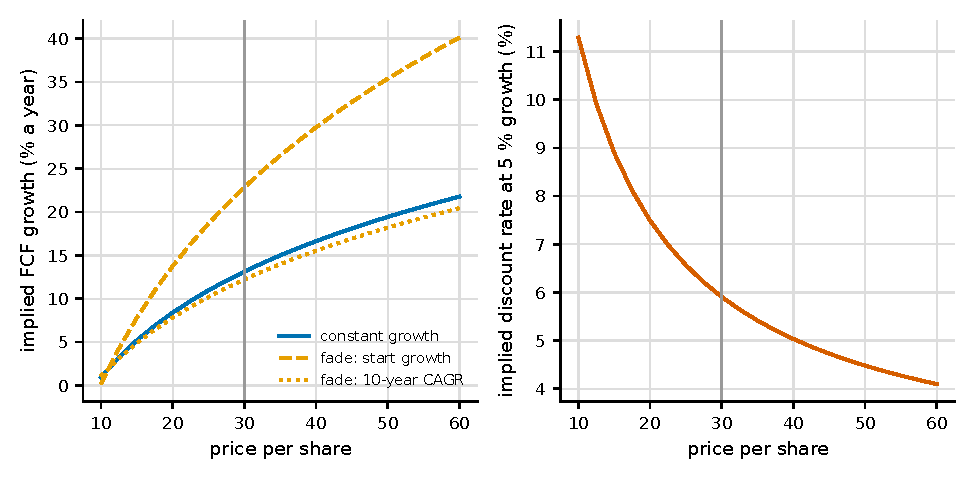
\includegraphics[width=0.74\linewidth]{figures/fig23_implied_growth.pdf}
\caption{Reverse DCF of the synthetic company (invented; FCF 100, discount rate 9\,\%, terminal growth 2\,\%, 10-year explicit period). Left: the FCF growth that a price implies - constant for 10 years, or the start growth of a linear fade to the terminal growth (dashed) with its 10-year CAGR (dotted). Right: the discount rate a price implies at a fixed 5\,\% growth. Grey line: the reference price 30.}
\label{fig:fig23_implied_growth}
\end{figure}

\begin{table}[H]
\centering
\scriptsize
\caption{Top: what a price implies (\%): the constant 10-year FCF growth, the start growth of a linear fade to the terminal growth with its 10-year CAGR, and the discount rate at a fixed 5\,\% growth. Bottom: the share of firms (\%, $\pm$ Monte-Carlo se) whose 10-year CAGR reaches the growth implied by the reference price, in the synthetic universe of the v0.4 survivorship study (2000 cohorts of 2000 firms; $\kappa$ = strength of growth-driven exits; survival in \%).}
\label{tab:D2_implied_growth}
\setlength{\tabcolsep}{5pt}
\begin{tabular}{lrrrr}
\toprule
Price & Constant & Fade start & Fade CAGR & Rate at 5\,\% \\
\midrule
10 & 0.97 & 0.17 & 1.08 & 11.29 \\
15 & 5.21 & 7.81 & 4.89 & 8.90 \\
20 & 8.41 & 13.77 & 7.82 & 7.49 \\
25 & 10.98 & 18.67 & 10.21 & 6.56 \\
30 & 13.14 & 22.86 & 12.23 & 5.91 \\
40 & 16.65 & 29.77 & 15.54 & 5.03 \\
50 & 19.44 & 35.38 & 18.21 & 4.48 \\
60 & 21.78 & 40.12 & 20.44 & 4.10 \\
\midrule
\textit{price 30} & \textit{survivors only} & \textit{full cohort} & \textit{counterfactual} & \textit{survival} \\
$\kappa$ = 0 & 14.3 $\pm$ 0.02 & 9.5 $\pm$ 0.01 & 14.4 $\pm$ 0.02 & 66.5 \\
$\kappa$ = 1 & 20.2 $\pm$ 0.03 & 10.4 $\pm$ 0.02 & 14.3 $\pm$ 0.02 & 51.8 \\
$\kappa$ = 2 & 36.7 $\pm$ 0.05 & 8.7 $\pm$ 0.01 & 14.3 $\pm$ 0.02 & 23.8 \\
\bottomrule
\end{tabular}
\end{table}

\begin{figure}[H]
\centering
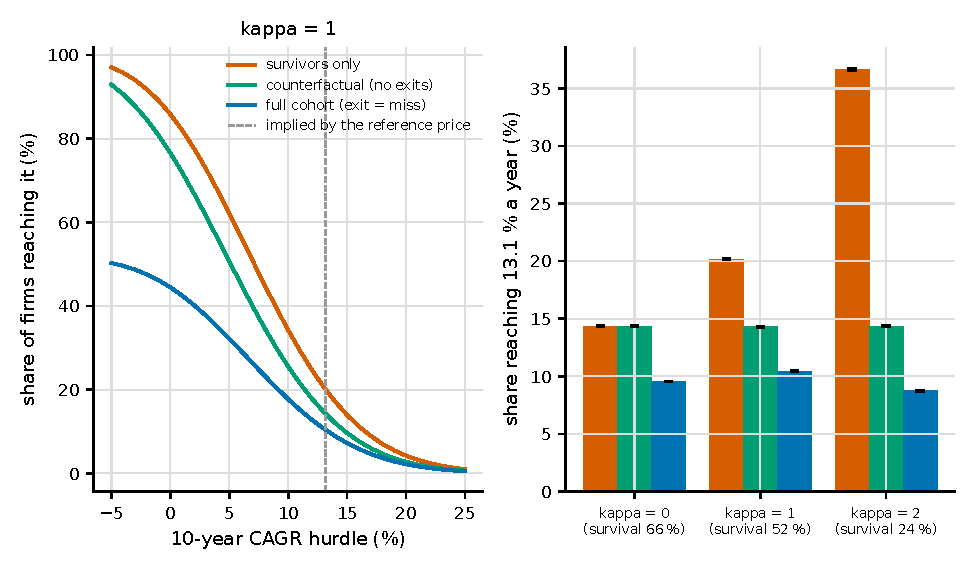
\includegraphics[width=0.74\linewidth]{figures/fig27_base_rates.pdf}
\caption{How often is the growth implied by the reference price achieved? Synthetic universe of the v0.4 survivorship study (2000 cohorts of 2000 firms, 10 years; FCF growth compared with revenue growth, i.e. a constant FCF margin assumed). Left: the three base rates against the CAGR hurdle (exit hazard strength kappa = 1). Right: at the implied growth, for exits unrelated to growth (kappa = 0) and increasingly growth-driven exits; error bars $\pm 1.96$ se. A database of today's survivors overstates the chance of a firm picked today.}
\label{fig:fig27_base_rates}
\end{figure}

\usertext{How the author would read the implied growth of a real company against base rates.}

% =====================================================================================
\section{Which assumptions decide}
\begin{figure}[H]
\centering
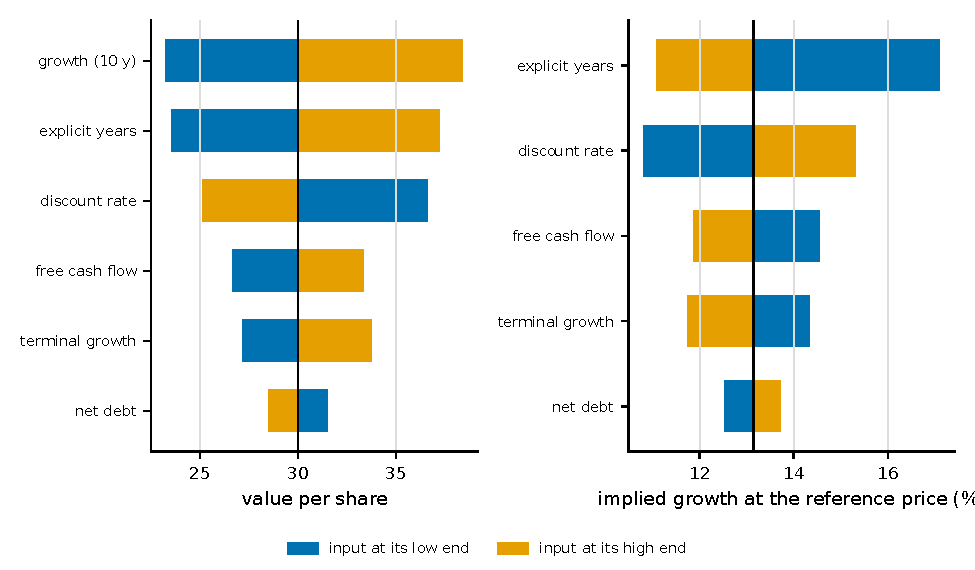
\includegraphics[width=0.74\linewidth]{figures/fig24_tornado.pdf}
\caption{One-way sensitivity (tornado) of the synthetic company, each input moved alone. Left: the value per share, at the growth the reference price implies (so the base value is the price). Right: the growth the reference price implies. Ranges: discount rate and terminal growth $\pm$1 percentage point, growth $\pm$3 points, FCF $\pm$10\,\%, net debt $\pm$50\,\%, explicit period 7--13 years.}
\label{fig:fig24_tornado}
\end{figure}

\begin{figure}[H]
\centering
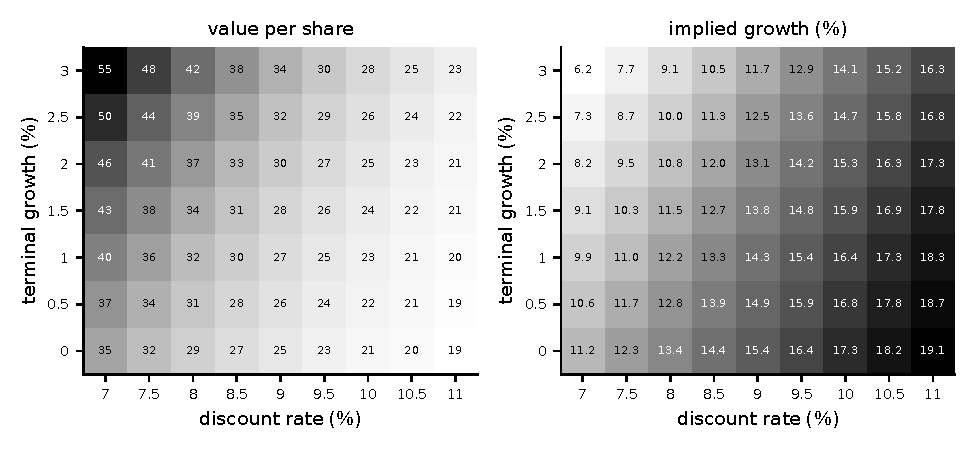
\includegraphics[width=0.74\linewidth]{figures/fig25_two_way.pdf}
\caption{Two-way sensitivity over the discount rate and the terminal growth (all other inputs at base). Left: value per share at the growth implied by the reference price (13.1\,\%); right: the growth the reference price 30 implies. Synthetic company.}
\label{fig:fig25_two_way}
\end{figure}

\begin{table}[H]
\centering
\scriptsize
\caption{One-way sensitivity (tornado), largest swing first; each input moved alone, all others at base. DCF: synthetic company at the reference price; the implied growth is re-solved for every input change. $\Delta$EVE: the v0.7 reference bank, non-maturity-deposit assumptions inside their caps. ECL: a 200-loan synthetic book with the v0.8 IFRS 9 model.}
\label{tab:D3_tornado}
\setlength{\tabcolsep}{4pt}
\begin{tabular}{lrrrr}
\toprule
Input & Range & Output at low & Output at high & Swing \\
\midrule
\textit{Value per share} &  &  &  &  \\
growth (10 y) & 10.14--16.14\,\% & 23.26 & 38.39 & 15.13 \\
explicit years & 7--13 & 23.56 & 37.20 & 13.63 \\
discount rate & 8.00--10.00\,\% & 36.59 & 25.11 & 11.49 \\
free cash flow & 90--110 & 26.65 & 33.35 & 6.70 \\
terminal growth & 1.00--3.00\,\% & 27.17 & 33.77 & 6.59 \\
net debt & 150--450 & 31.50 & 28.50 & 3.00 \\
\midrule
\textit{Implied growth (\%)} &  &  &  &  \\
explicit years & 7--13 & 17.11 & 11.08 & 6.03 \\
discount rate & 8.00--10.00\,\% & 10.80 & 15.31 & 4.51 \\
free cash flow & 90--110 & 14.55 & 11.87 & 2.69 \\
terminal growth & 1.00--3.00\,\% & 14.34 & 11.74 & 2.60 \\
net debt & 150--450 & 12.53 & 13.73 & 1.20 \\
\midrule
\textit{Worst $\Delta$EVE / Tier 1 (\%)} &  &  &  &  \\
current accounts: avg.\ maturity & 1--5 & 29.08 & 8.42 & 20.66 \\
current accounts: core share & 50--90\,\% & 22.87 & 12.32 & 10.55 \\
savings: avg.\ maturity & 1--4.5 & 19.06 & 14.51 & 4.55 \\
savings: core share & 30--70\,\% & 18.85 & 16.34 & 2.51 \\
\midrule
\textit{ECL coverage (\%)} &  &  &  &  \\
LGD scale & 0.8--1.2 & 0.748 & 1.122 & 0.374 \\
current PD scale & 0.8--1.2 & 0.768 & 1.121 & 0.353 \\
SICR multiple & 2--4 & 1.115 & 0.920 & 0.194 \\
downside weight & 0.1--0.5 & 0.843 & 1.027 & 0.184 \\
downside severity & 0.5--1.5 & 0.866 & 1.003 & 0.138 \\
\bottomrule
\end{tabular}
\end{table}

The tornado moves one input at a time and therefore shows neither interactions nor the shape between the ends. The
Sobol indices below cover the joint uncertainty; their size depends on the ranges chosen, which are part of the
result (Table~\ref{tab:D5_assumptions}).

\subsection{The same tools on other Risk Lab models}
For the synthetic bank of the IRRBB study the output is the worst decline of the economic value of equity over the six
standard shocks, as a share of Tier 1, and the inputs are the non-maturity-deposit assumptions (core share and average
maturity of current accounts and savings, inside the regulatory caps). For the credit study the output is the ECL
coverage of a 200-loan book, and the inputs are the downside-scenario weight and severity, the SICR threshold and
scalings of LGD and current PD. Both appear in Tables~\ref{tab:D3_tornado} and \ref{tab:D4_sobol} and in
Figure~\ref{fig:fig26_sobol}.
\usertext{What these cross-checks mean for the model-risk inventory of the IRRBB and ECL models.}

\begin{figure}[H]
\centering
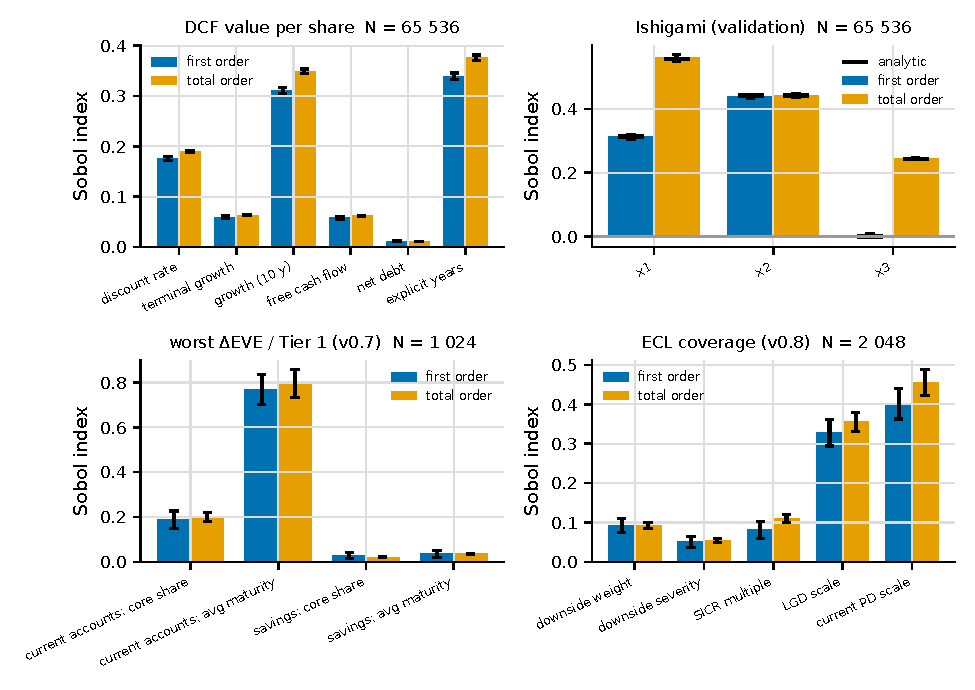
\includegraphics[width=0.66\linewidth]{figures/fig26_sobol.pdf}
\caption{Variance-based (Sobol) sensitivity indices: first order (the input alone) and total order (with all interactions), Saltelli sampling with the Jansen total-order estimator, error bars $\pm 1.96$ bootstrap se. Top left: the synthetic company's value per share over the six inputs and ranges of the tornado (the explicit period discrete uniform over 7--13 years). Top right: the Ishigami function, where the analytic indices (black marks) are known - a check of the estimator. Bottom: the same tool on the v0.7 bank (non-maturity-deposit assumptions) and on a v0.8 loan book (scenario weight and severity, SICR threshold, LGD and PD scaling).}
\label{fig:fig26_sobol}
\end{figure}

\begin{table}[H]
\centering
\scriptsize
\caption{Sobol indices (first order: the input alone; total order: with all its interactions), N base rows ($N(k+2)$ runs), $\pm$ bootstrap se; independent uniform inputs over the ranges of Tab.~\ref{tab:D5_assumptions} (DCF: the tornado's six inputs, the explicit period over whole years 7--13). A first-order index above its total (savings core share, $\Delta$EVE) is Monte-Carlo noise; in theory $S_i \le S_{Ti}$.}
\label{tab:D4_sobol}
\setlength{\tabcolsep}{5pt}
\begin{tabular}{lrrr}
\toprule
Input & First order & Total order & Analytic first / total \\
\midrule
\textit{DCF value per share}\, N = 65\,536 &  &  &  \\
discount rate & 0.176 $\pm$ 0.002 & 0.190 $\pm$ 0.001 &  \\
terminal growth & 0.059 $\pm$ 0.001 & 0.063 $\pm$ 0.000 &  \\
growth (10 y) & 0.311 $\pm$ 0.003 & 0.349 $\pm$ 0.002 &  \\
free cash flow & 0.058 $\pm$ 0.001 & 0.062 $\pm$ 0.000 &  \\
net debt & 0.011 $\pm$ 0.001 & 0.011 $\pm$ 0.000 &  \\
explicit years & 0.339 $\pm$ 0.003 & 0.377 $\pm$ 0.003 &  \\
\midrule
\textit{Ishigami (analytic check)}\, N = 65\,536 &  &  &  \\
$x_1$ & 0.314 $\pm$ 0.004 & 0.560 $\pm$ 0.005 & 0.314 / 0.558 \\
$x_2$ & 0.440 $\pm$ 0.003 & 0.442 $\pm$ 0.003 & 0.442 / 0.442 \\
$x_3$ & 0.003 $\pm$ 0.003 & 0.246 $\pm$ 0.002 & 0.000 / 0.244 \\
\midrule
\textit{worst $\Delta$EVE / Tier 1 (v0.7)}\, N = 1\,024 &  &  &  \\
current accounts: core share & 0.188 $\pm$ 0.020 & 0.199 $\pm$ 0.011 &  \\
current accounts: avg.\ maturity & 0.770 $\pm$ 0.034 & 0.794 $\pm$ 0.031 &  \\
savings: core share & 0.030 $\pm$ 0.006 & 0.021 $\pm$ 0.001 &  \\
savings: avg.\ maturity & 0.036 $\pm$ 0.008 & 0.035 $\pm$ 0.002 &  \\
\midrule
\textit{ECL coverage (v0.8)}\, N = 2\,048 &  &  &  \\
downside weight & 0.092 $\pm$ 0.009 & 0.091 $\pm$ 0.004 &  \\
downside severity & 0.051 $\pm$ 0.007 & 0.054 $\pm$ 0.002 &  \\
SICR multiple & 0.081 $\pm$ 0.011 & 0.111 $\pm$ 0.005 &  \\
LGD scale & 0.328 $\pm$ 0.017 & 0.355 $\pm$ 0.012 &  \\
current PD scale & 0.401 $\pm$ 0.020 & 0.455 $\pm$ 0.017 &  \\
\bottomrule
\end{tabular}
\end{table}

\usertext{Which input ranges the author would defend for a real company, and which inputs deserve the most work.}

% =====================================================================================
\section{Limitations}
\begin{itemize}
\item Synthetic example: the company, the universe and all ranges are invented; the numbers illustrate the methods.
\item Simple DCF: end-of-year cash flows, a single discount rate, no explicit reinvestment or margin model; the
  terminal value carries most of the value.
\item Base rates: revenue-growth universe as a proxy for free-cash-flow growth (constant margin); its parameters are
  modelling choices.
\item Sobol indices assume independent inputs and describe the variance over the stated ranges only; plain Monte Carlo
  with bootstrap errors (no quasi-random sequences); the estimators follow Saltelli et al.\ (2010) and Jansen (1999)
  and are validated on analytic test functions.
\end{itemize}
\usertext{Further limitations the author sees.}

% =====================================================================================
\section{Assumptions register}
\begin{table}[H]
\centering
\scriptsize
\caption{Assumptions register of the valuation study (``ASSUMPTION'' = not verified against a primary source in this work, or a modelling assumption the result depends on; ``stated'' = a modelling choice or a cited textbook method).}
\label{tab:D5_assumptions}
\setlength{\tabcolsep}{3pt}
\begin{tabular}{>{\raggedright\arraybackslash}p{3.0cm}>{\raggedright\arraybackslash}p{10.6cm}>{\raggedright\arraybackslash}p{2.1cm}}
\toprule
Item & Statement and source & Status \\
\midrule
Sobol inputs & independent and uniform (a modelling choice; the DCF explicit period discrete uniform over whole years); the DCF ranges equal the tornado ranges; the indices describe the variance over these ranges, not the world & stated \\
Sobol ranges (DCF) & discount\_rate U(0.08, 0.1); fcf0 U(90, 110); growth U(0.1014, 0.1614); net\_debt U(150, 450); terminal\_growth U(0.01, 0.03); years U(7, 13) & stated \\
Sobol ranges (ECL) & downside\_severity U(0.5, 1.5); downside\_weight U(0.1, 0.5); lgd\_scale U(0.8, 1.2); pd\_scale U(0.8, 1.2); sicr\_multiple U(2, 4) & stated \\
Sobol ranges (IRRBB) & ca\_avg\_maturity U(1, 5); ca\_core\_share U(0.5, 0.9); sav\_avg\_maturity U(1, 4.5); sav\_core\_share U(0.3, 0.7) & stated \\
Sobol sampling & plain Monte Carlo (not quasi-random) so that the bootstrap error is valid; first-order estimator with outputs centred by their mean (numerical-stability variant: same estimand, O(1/N) bias, lower variance) & stated \\
base-rate proxy & FCF growth compared with the revenue growth of the synthetic universe: assumes a constant FCF margin - ASSUMPTION of the comparison & ASSUMPTION \\
cash-flow timing & end of year (no mid-year convention); terminal value by the Gordon growth formula & stated \\
company & synthetic, invented with round numbers; not a real company and not calibrated to market data; for a real company the inputs are user-provided at run time & stated \\
source: base rates & synthetic universe of the v0.4 survivorship study (same draws); FCF growth compared with revenue growth assumes a constant FCF margin (modelling assumption) & stated \\
source: dcf & enterprise DCF with Gordon terminal value (textbook: Koller, Goedhart and Wessels, Valuation; Damodaran, Investment Valuation); end-of-year cash flows & stated \\
source: reverse DCF & price as given, solve for the implied growth (Mauboussin and Rappaport, Expectations Investing); Brent root finding on an explicit bracket & stated \\
source: sobol & Sobol' (2001); estimators of Saltelli et al. (2010, Comput. Phys. Commun. 181, 259-270) Table 2: first order (b), total order (f) = Jansen (1999); confirmed in the v0.9 review (consistent with SALib) and checked against the analytic Ishigami indices; the first-order estimator uses centred outputs (numerical-stability variant, same estimand, O(1/N) bias) & stated \\
\bottomrule
\end{tabular}
\end{table}


\section{Findings}
\begin{table}[H]
\centering
\scriptsize
\caption{Findings register of the valuation study. Severities are PROPOSED and must be confirmed by the validator.}
\label{tab:D6_findings}
\setlength{\tabcolsep}{3pt}
\begin{tabular}{>{\raggedright\arraybackslash}p{0.75cm}>{\raggedright\arraybackslash}p{6.6cm}>{\raggedright\arraybackslash}p{1.85cm}>{\raggedright\arraybackslash}p{2.4cm}>{\raggedright\arraybackslash}p{3.5cm}}
\toprule
ID & Finding & Severity & Evidence & Proposed remediation \\
\midrule
D-F1 & The reference price 30 implies 13.1\,\% FCF growth a year for 10 years. In the synthetic universe ($\kappa$ = 1) 20.2 $\pm$ 0.03\,\% of today's survivors reached that, but only 10.4 $\pm$ 0.02\,\% of the firms alive at the start: a survivors-only base rate overstates the chance by a factor 1.9 (factor 4.2 with strongly growth-driven exits, $\kappa$ = 2). & PROPOSED: High & Tab.~\ref{tab:D2_implied_growth}; Fig.~\ref{fig:fig27_base_rates} & Judge an implied growth against full-cohort base rates (exits counted as misses), not against databases of current constituents. \\
D-F2 & The implied growth is not a market fact but conditional on unobservable inputs: the explicit period (7 vs 13 years) moves it from 17.1 to 11.1\,\%, the discount rate (8 vs 10\,\%) from 10.8 to 15.3\,\%; the terminal value is 63\,\% of the enterprise value. & PROPOSED: Medium & Tab.~\ref{tab:D3_tornado}; Fig.~\ref{fig:fig24_tornado}, \ref{fig:fig25_two_way} & Report the implied growth with its sensitivity to the discount rate, the horizon and the terminal growth, never as a single number. \\
D-F3 & Over the tornado's ranges (including the explicit period, discrete uniform 7--13 years) the DCF value is driven by the explicit period (total index 0.38), the growth (0.35) and the discount rate (0.19); terminal growth and FCF contribute 0.06 and 0.06, net debt 0.011. The first-order indices sum to 0.95; the largest first / total gaps are those of the growth and the explicit period (about 0.04 each), consistent with their interaction (growth compounds over the period). & PROPOSED: Low & Tab.~\ref{tab:D4_sobol}; Fig.~\ref{fig:fig26_sobol} & State the input ranges with every index: the ranking depends on them. \\
D-F4 & Applied to the v0.7 bank, the average maturity of the current-account deposits alone explains 0.77 $\pm$ 0.03 of the variance of the worst $\Delta$EVE / Tier 1 (total 0.79); within the caps it moves the ratio from 8.4 to 29.1\,\% of Tier 1, across the 15\,\% outlier threshold. & PROPOSED: Medium & Tab.~\ref{tab:D3_tornado}, \ref{tab:D4_sobol} & Validate and disclose the NMD maturity assumption first; it decides the outlier test. \\
D-F5 & For the v0.8 ECL, current-PD and LGD scaling dominate (total 0.455 $\pm$ 0.017 and 0.355 $\pm$ 0.012). The SICR multiple has a first-order index of 0.081 $\pm$ 0.011 and a total index of 0.111 $\pm$ 0.005 (N = 2\,048): the gap of 0.03 is about 3 first-order se: a modest interaction (plausibly with the PD level), not conclusive. Staging is the v0.8 same-basis rule (scenarios change the amount, not the stage). & PROPOSED: Low & Tab.~\ref{tab:D3_tornado}, \ref{tab:D4_sobol} & Use global (Sobol) sensitivity for models with thresholds and report the errors with the indices. \\
D-F6 & The Sobol estimators (Saltelli et al. 2010 (b), Jansen 1999; confirmed in the review, consistent with SALib) reproduce the analytic Ishigami indices within Monte-Carlo error (largest deviation 1.1 bootstrap se, N = 65\,536); centred first order: same estimand, O(1/N) bias. & PROPOSED: Low & Tab.~\ref{tab:D4_sobol}; Fig.~\ref{fig:fig26_sobol} & Keep the analytic test cases in the test suite. \\
D-F7 & The base rates come from a synthetic revenue-growth universe; comparing FCF growth with it assumes a constant FCF margin, and the universe's parameters (drift, volatility, exit hazard) are modelling choices, not calibrations. & PROPOSED: Low & Tab.~\ref{tab:D5_assumptions} & For a real decision, use a full-cohort database (including delisted firms) of the relevant metric. \\
\bottomrule
\end{tabular}
\end{table}


\section*{References}
\vspace{-0.5em}
\begin{itemize}\footnotesize\setlength{\itemsep}{0pt}\setlength{\parskip}{0pt}
\item Koller, T., Goedhart, M. and Wessels, D. \emph{Valuation}. Wiley.
\item Damodaran, A. \emph{Investment Valuation}. Wiley; Mauboussin, M. J. and Rappaport, A. \emph{Expectations Investing}. Harvard Business School Press.
\item Sobol', I. M. (2001). Global sensitivity indices for nonlinear mathematical models and their Monte Carlo
  estimates. \emph{Mathematics and Computers in Simulation} 55, 271--280.
\item Jansen, M. J. W. (1999). Analysis of variance designs for model output. \emph{Computer Physics Communications}
  117, 35--43.
\item Saltelli, A., Annoni, P., Azzini, I., Campolongo, F., Ratto, M. and Tarantola, S. (2010). Variance based
  sensitivity analysis of model output. Design and estimator for the total sensitivity index. \emph{Computer Physics
  Communications} 181, 259--270.
\item Ishigami, T. and Homma, T. (1990). An importance quantification technique in uncertainty analysis for computer
  models. \emph{Proceedings of ISUMA '90}.
\end{itemize}


\end{document}
